\documentclass{beamer}
%% Possible paper sizes: a0, a0b, a1, a2, a3, a4.
%% Possible orientations: portrait, landscape
%% Font sizes can be changed using the scale option.
\usepackage[size=a3,orientation=portrait,scale=1.8]{beamerposter}
\usetheme{LLT-poster}
\usecolortheme{ComingClean}
% \usecolortheme{Entrepreneur}
% \usecolortheme{ConspiciousCreep}  %% VERY garish.

\usepackage[utf8]{inputenc}
\usepackage[T1]{fontenc}
\usepackage{libertine}
\usepackage[scaled=0.92]{inconsolata}
\usepackage[libertine]{newtxmath}
\usepackage[numbers]{natbib}
\renewcommand{\bibfont}{\small}

\newcommand{\texthash}{\#}


%% Load the markdown package
\usepackage[citations,footnotes,definitionLists,hashEnumerators,smartEllipses,tightLists=false,pipeTables,tableCaptions,hybrid]{markdown}
%%begin novalidate
\markdownSetup{rendererPrototypes={
 link = {\href{#2}{#1}},
 headingFour = {\begin{block}{#1}},
 horizontalRule = {\end{block}}
}}
%%end novalidate

\author[tkoyama@gmail.com]{Tetsuo Koyama}
\title{PyVista: A Python Library for Interactive 3D Data Visualization and Analysis}
\institute{PyVista community}
% Optional foot image
\footimage{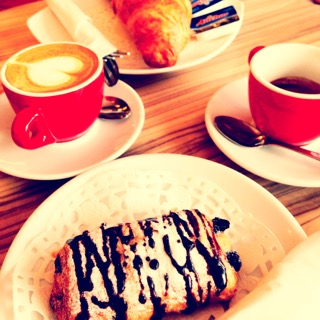
\includegraphics[width=4cm]{IMG_1934.jpg}}

\begin{document}
\begin{frame}[fragile]\centering

\begin{columns}
\begin{column}{1.0\textwidth}

\begin{markdown}

#### Abstract

This poster showcases the powerful features of PyVista, a Python library for 3D data visualization and analysis.

We demonstrate PyVista's ability to create interactive 3D visualizations, process, and filter point cloud data, perform advanced modeling and analysis, and more.
We also highlight PyVista's ease of use and flexibility, making it an excellent tool for anyone working with 3D data.
Our poster includes code examples and visualizations to demonstrate PyVista's capabilities and provide practical applications for users.

Our poster is a great resource for those looking to enhance their 3D data analysis and visualization workflows using PyVista.

----
\end{markdown}
\end{column}

\end{columns}

\bigskip
{\usebeamercolor[bg]{headline}\hrulefill}
\bigskip

\begin{columns}[T]

%%%% First Column
\begin{column}{.46\textwidth}

\begin{markdown}

#### Overview

* This is the template I created for my poster presentations. [@novotny:2017]
* You can provide an optional \texttt{\textbackslash footimage}. [@novotny:2019]

----


#### Options

* It's based on \texttt{beamerposter}, so you can change some options:

    size
    
    :   a0, a0b, a1, a2, a3, a4

    orientiation
    
    :   landscape, portrait
    
    scale
    :   a decimal number to scale the fonts

----

#### Colour Themes

- I've included some colour themes, using the colour palettes from \url{http://colourlovers.com}
    * ComingClean (current theme)
    * Entrepreneur (light blue + grey)
    * Conspicious (a bit garish!)

---- 

#### Figures and images

\setkeys{Gin}{width=.3\linewidth}

![exampleimage](example-image.jpg "An exemplary image")

----

\end{markdown}

\end{column}

%%%% Second Column
\begin{column}{.46\textwidth}

\begin{markdown}

#### This is a sample

- One, two, pick up my shoe
- Three, four, shut the door
- Five, six, pick up sticks
- Seven, eight, lay them straight
- Nine, ten, a big fat hen
- One, two, pick up my shoe
- Three, four, shut the door
- Five, six, pick up sticks
- Seven, eight, lay them straight
- Nine, ten, a big fat hen

----

#### This is another sample

- Some maths material

\begin{align}
A &= U \times S \times V^T\\
\sigma &= \frac{x\times y}{\sqrt[3]{\alpha + \beta}}
\end{align}

----


#### `pipeTables` and `tableCaptions`

| Right | Left | Default | Center |
|------:|:-----|---------|:------:| 
|  12   |  12  |  12     |   12   | 
| 123   |  123 |   123   |  123   | 
|   1   |    1 |     1   |    1   | 

  : Demonstration of pipe table syntax.

----

\end{markdown}
\end{column}
\end{columns}

\begin{markdown}

#### This is a sample of a wiiiide column

- One, two, pick up my shoe
- Three, four, shut the door
- Five, six, pick up sticks

----

#### Bibliography

\bibliographystyle{unsrtnat}
\bibliography{refs}

----

\end{markdown}

\end{frame}


\end{document}
